\section{Method}
\label{sec:method}
\begin{figure*}
\vspace{-24pt}
\centering
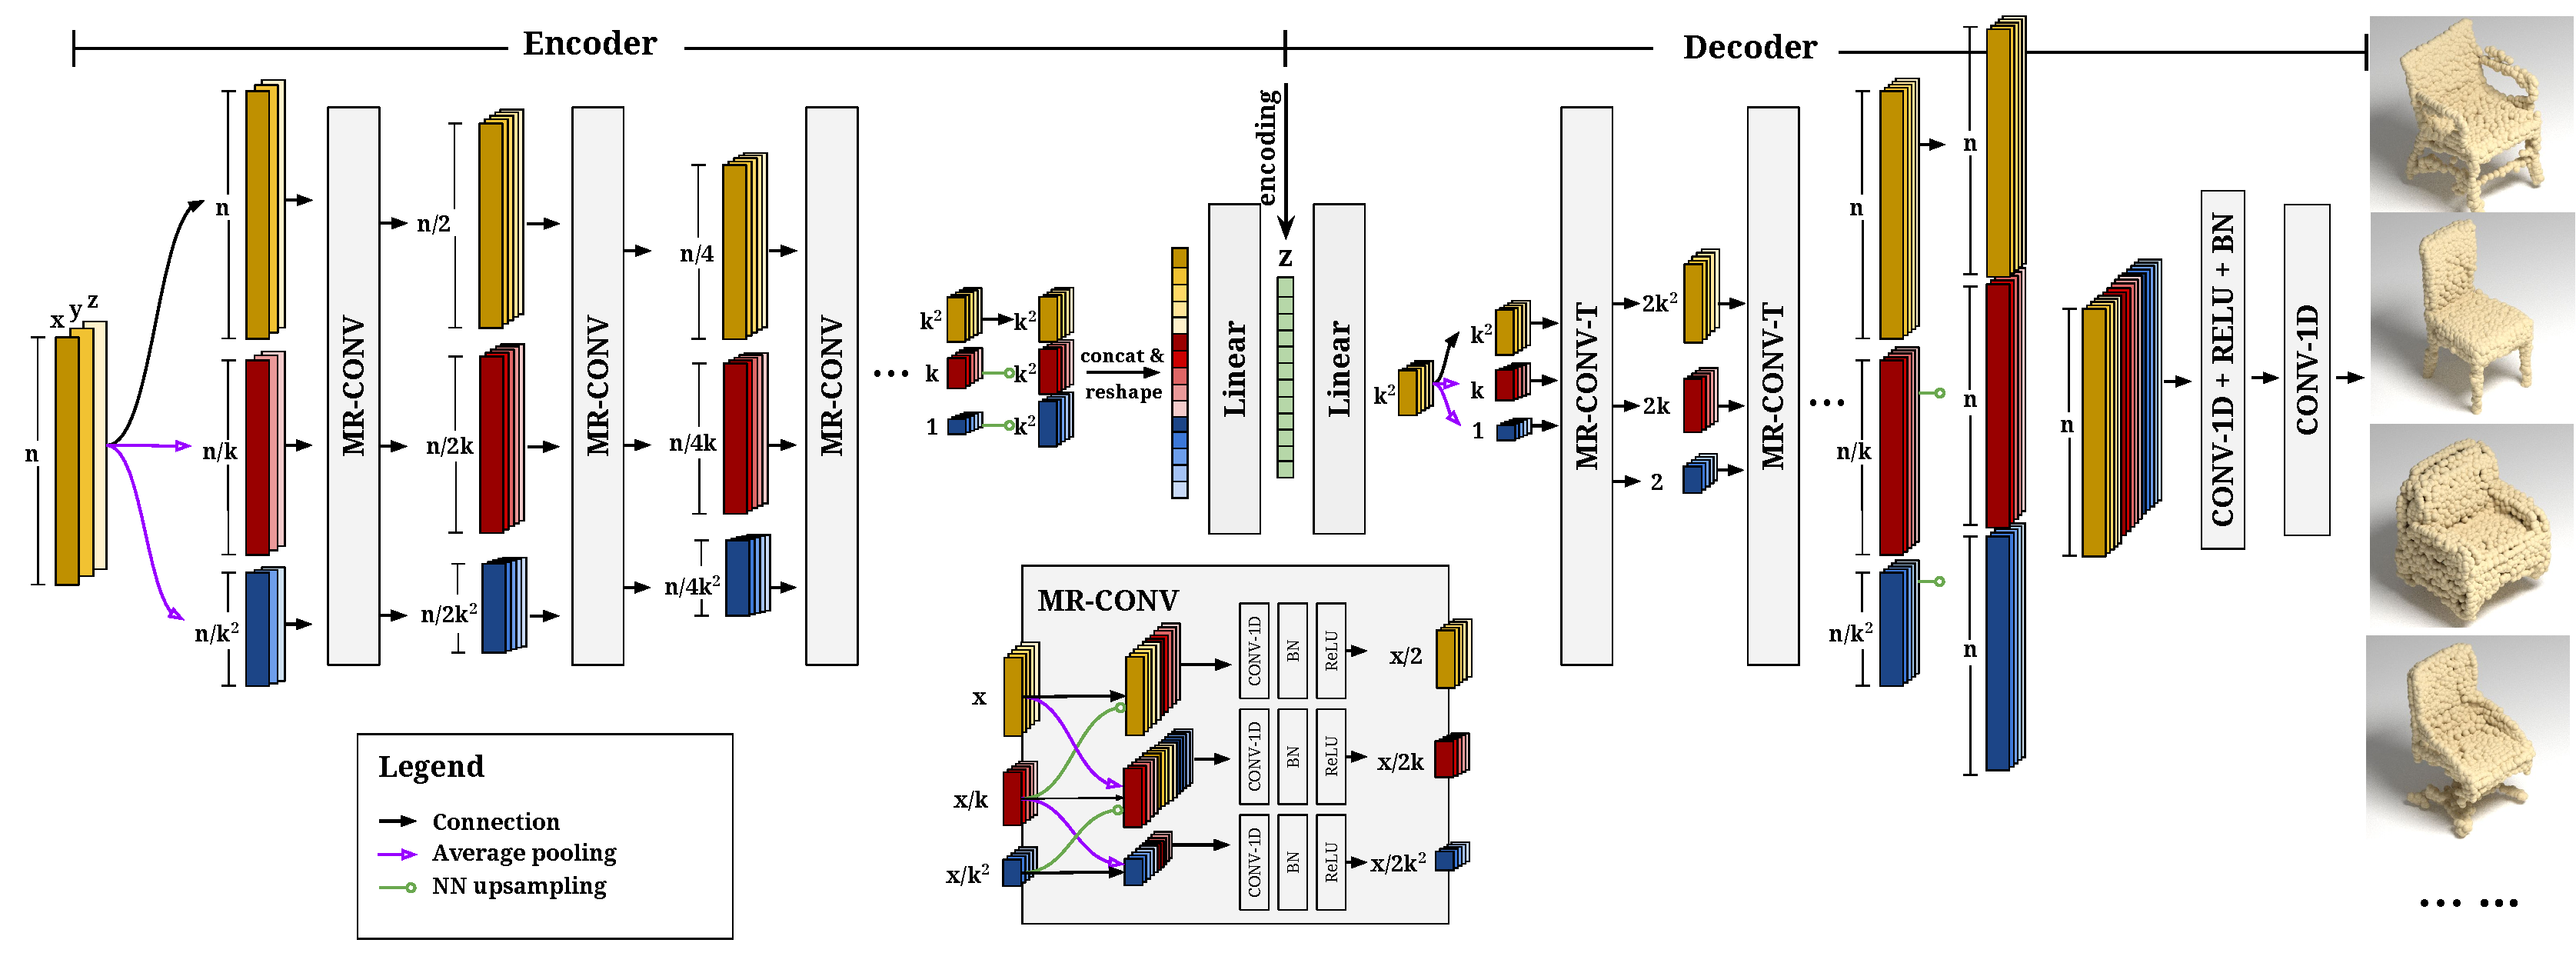
\includegraphics[width=1.0\linewidth]{MRTNet/imgs/MultiresArchitecture.pdf}
\vspace{-20pt}
	\caption{\small \label{fig:multires-arch} Our multiresolution tree network (\mrtnet) for processing 3D point clouds. We represent a 3D shape as a 1D list of spatially sorted point cloud. The network represents each layer at three scales (indicated by yellow, red, and blue), the scale ratio is $k$ between each two. The last two convolution layers have kernel size 1 and stride 1. MR-CONV refers to multi-resolution convolution (zoom-in to the inset for details); and MR-CONV-T refers to MR-CONV with transposed convolution. Our network is flexible and can be used for several shape processing tasks.}
\vspace{-16pt}
\end{figure*}
Figure~\ref{fig:multires-arch} shows the complete architecture of our multiresolution tree network (\mrtnet) that includes both the encoder and decoder.
We represent 3D shapes as a point cloud of a fixed size $\npoints=2^\depth$ (e.g. $\npoints=1K$). We center the point cloud at the origin and normalize its bounding box; then spatially sort it using a space-partitioning tree. The input to the network are thus a 1D list ($\npoints \times 3$ tensor) containing the $xyz$ coordinates of the points. The network leverages 1D convolution and represents each layer at three scales, with a ratio of $\scale$ between each two. MR-CONV refers to multi-resolution convolution, and MR-CONV-T refers to MR-CONV with transposed convolution. The encoding $\encoding$ is a 512-D vector. 
Our network architecture is flexible and can be used for several shape processing tasks. For shape \textbf{classification}, 
we use only the multiresolution encoder but adding a fully connected layer after the encoding $\encoding$ to output a 40-D vector representing the ModelNet40 shape classes. 
For \textbf{single-image shape inference}, we employ a pretrained VGG-11 image encoder~\cite{vgg}, 
combined with our multiresolution decoder to directly an output point cloud shape as a $\npoints \times 3$ tensor. 
For \textbf{unsupervised learning of point clouds}, we use both the multiresolution encoder and decoder, forming a variational autoencoder. 


\para{Spatial sorting.} As a point cloud is unordered to begin with, we use a space-partitioning tree such as KD-tree to order the points. To start, we sort the entire point set along the $x$-axis, then split it in half, resulting in equal-sized left and right subsets; we then recursively split each subset, this time along the $y$-axis; then along $z$-axis; then back along the $x$-axis and so on. Basically it's a recursive process to build a full tree where the splitting axes alternate between $x$, $y$, $z$ at each level of the tree. The order of leaf nodes naturally becomes the order of the points. There are several variants on the splitting strategy. If at each split we choose an axis among $x$, $y$, $z$ with probability proportional to the span of the subset along that axis, it builds a probabilistic KD-tree as described in~\cite{Klokov_2017_ICCV}. If we choose axes from a random set of directions, it builds an RP-tree~\cite{Dasgupta:2008:RPT}.
Note that after the ordering is obtained, the underlying details of the how the splits were taken are discarded.
This is fundamentally different from~\cite{Klokov_2017_ICCV} where the network computations are conditioned on the splitting directions.



The purpose of spatial sorting is to build a hierarchical and locality-preserving order of the points.
Thus functions computed based on the local 3D neighborhood at a point can be approximated using convolutions and pooling operations on the 1D structure.
However, any ordering of points is distortion inducing and in particular long-range relationships are not preserved well.
Maintaining multiple resolutions of the data allows us to preserve locality at different scales.
Since the partitioning is constructed hierarchically this can be efficiently implemented using pooling operations described next.






\para{Multiresolution convolution.} With the spatially sorted point set, we can build a network using 1D convolution and pooling operations. The convolution leverages the spatial locality of points after sorting, and the pooling leverages the intrinsic binary tree structure of the points. %



With a conventional CNN, each convolutional operation has a restricted receptive field and is not able to leverage both global and local information effectively. We resolve this issue by maintaining three different resolutions of the same point cloud using a mutligrid architecture~\cite{multigrid}. Different resolutions are computed directly through pooling and upsampling operations. Specifically, we use average pooling with kernel size and stride of $k$, where $k$ is a power of 2. This configuration allows pooling/downsampling the point cloud while preserving its hierarchical tree structure. Figure~\ref{fig:multires-abs} (left) shows an example point cloud at three different resolutions computed by pooling with $k=2$. For upsampling, we use nearest neighbor (NN) upsampling with a factor of $k$.

Once we can pool and upsample the point clouds, we are able to combine global and local information
in the convolutional operations by using the MR-CONV block in the inset of Fig.~\ref{fig:multires-arch}.
The multiresolution block operates in the following way.
We maintain the point cloud representations at three resolutions $\mathbf{f}_{(0)}$, $\mathbf{f}_{(1)}$, $\mathbf{f}_{(2)}$,
where the scale ratio between each two is (as mentioned above) $k$.
The MR-CONV block receives all three as input, and each resolution will be upsampled and/or pooled and concatenated with each other, creating three new representations 
$\mathbf{f}^\prime_{(0)}$, $\mathbf{f}^\prime_{(1)}$, $\mathbf{f}^\prime_{(2)}$:
\begin{equation}
\mathbf{f}^\prime_{(0)} = \mathbf{f}_{(0)} \oplus up(\mathbf{f}_{(1)}); \quad \mathbf{f}^\prime_{(1)} = pool(\mathbf{f}_{(0)}) \oplus \mathbf{f}_{(1)} \oplus up(\mathbf{f}_{(2)}); \quad \mathbf{f}^\prime_{(2)} = pool(\mathbf{f}_{(1)}) \oplus \mathbf{f}_{(2)}. \nonumber
\end{equation}
where $\oplus$ is the concatenation operation, $up$ and $pool$ are the upsampling
and average pooling operations.
Each new representation $\mathbf{f}^\prime$ then goes through a sequence of operations: 1D convolution (kernel size=2 and stride=2), batch normalization and ReLU activation.
Note that due to the stride 2, each output is half the size of its associated input.
In our generative model and shape inference model we use $k=4$, while for classification we use $k=8$.

\para{Shape classification model.} For classification, we use our multiresolution encoder in Figure~\ref{fig:multires-arch}, and add a fully connected layer after encoding $\mathbf{z}$ that outputs a 40-D vector representing the ModelNet40 classification. Specifically, we train the network on the ModelNet40~\cite{wu20153d} dataset, which contains 12,311 objects covering 40 different categories. It is split into 9,843 shapes for training and 2,468 shapes for testing. For each object, we sample 1K points on the surface using Poisson Disk sampling~\cite{Bowers:2010:PPD} to evenly disperse the points. Each sampled point cloud is then spatially sorted using the probabilistic kd-tree~\cite{Klokov_2017_ICCV}. Specifically, at each split of the tree we choose a random split axis according to the following PDF:
\begin{equation}
	P(\mathbf{n}=\mathbf{e}_i | \mathbf{x}) = \frac{\exp\{span_i(\mathbf{x})\}}{\sum_{j=1}^{d}\exp\{span_j(\mathbf{x})\}} \nonumber
\end{equation}
where $\mathbf{x}$ is the subset of points to be split, $\mathbf{n}$ is the split axis chosen from the canonical axes $\mathbf{e}_i$ (i.e. $x$,$y$,$z$ in 3D), and $span_i(\mathbf{x})$ returns the span of $\mathbf{x}$ along each axis $\mathbf{e}_i$.

The network parameters are as follows: the first MR-CONV layer has 16 filters and the following layers double the amount of filter of the previous one, unless the previous layer has 1024 filters. In that case, the next layer also has 1024 filters. The network is trained by minimizing a cross-entropy loss using an Adam optimizer with learning rate $10^{-3}$ and $\beta = 0.9$. The learning rate is decayed by dividing it by 2 every 5 training epochs. We employ scale augmentation at training and test time by applying anisotropic scaling factors drawn from $\mathcal{N}(1, 0.25)$.
At test time, for each point cloud we apply the sampled scale factors and build the probabilistic kd-tree 16 times as described above, thus obtaining 16 different versions and orderings of the point set.
Our final classification is the mean output of those versions. The test-time average has very little impact on the computation time (a discussion is included in Sec.~\ref{sec:discussions}). 


\para{Single-image shape inference.} Our multiresolution decoder can be used to perform image-to-shape inference. 
Specifically, we use a pretrained VGG-11 image encoder~\cite{vgg} combined with our decoder in Figure~\ref{fig:multires-arch}. 
Our decoder is set to generates 4K points. 
The entire network is trained using the dataset and splits provided by~\cite{choy20163d}, 
which contains 24 renderings from different views for 43783 shapes from ShapeNet divided in 13 different categories. 
We sample each ShapeNet mesh at 4K points and use them for supervision.
Given a rendered image, the task is to predict the complete point cloud (4K points) representing the object in the image.
The decoder in Figure~\ref{fig:multires-arch} has the following number of filters per layer:
512-512-256-256-128-64-64-64. As in Figure~\ref{fig:multires-arch}, the two additional
convolutional layers at the end have kernel size 1 and stride 1: the first one has 128 filters and the second one outputs the final 4K point set.

There are many possible choices for the reconstruction loss function. One straightforward choice would be to use the ordering induced by the spatial partitioning and compute the $L_2$ loss between the output and ground-truth point clouds. However, $L_2$ loss turns out to work very poorly. 
We chose to use the Chamfer distance between two point clouds ($\mathbf{x}$ and $\mathbf{y}$), defined as:
\begin{equation}
	Ch(\mathbf{x}, \mathbf{y})=
		 \frac{1}{|\mathbf{x}|}\sum_{x \in \mathbf{x}} \min_{y \in \mathbf{y}} \norm{x-y}_2 +
		 \frac{1}{|\mathbf{y}|}\sum_{y \in \mathbf{y}} \min_{x \in \mathbf{x}} \norm{x-y}_2 \nonumber
\end{equation}
The Chamfer distance is invariant to permutations of points, making it suitable to measure dissimilarities between unstructured point clouds.
The model is trained using an Adam optimizer with learning rate $10^{-3}$ and $\beta = 0.9$.
Learning rate is divided by two at each two epochs.

\para{Unsupervised learning of point clouds.} By combining the multiresolution encoder and decoder together, we can perform unsupervised learning of 3D shapes. The entire network, called \mrvae, builds upon a variational autoencoder (VAE) \cite{vae} framework. %
The encoder $Q$ receives as an input a point cloud $\mathbf{x}$ and outputs an encoding $\mathbf{z} \in \mathbb{R}^{512}$. The decoder $D$ tries to replicate the point cloud $\mathbf{x}$ from $\mathbf{z}$. Both encoder and decoder are built using a sequence of MR-CONV blocks as in Fig.~\ref{fig:multires-arch}. Similar to above, we use Chamfer distance as the reconstruction loss function. Besides this, we also need a regularization term that forces the distribution
of the encoding $\mathbf{z}$ to be as close as possible to the Gaussian $\mathcal{N}(0,I)$. Differently from the original VAE model, we found that we can get more stable training if we try to match the first two moments (mean and variance) of $\mathbf{z}$ to $\mathcal{N}(0,I)$. Mathematically, this regularization term is defined as:
\begin{equation}
	\mathcal{L}_{reg} = \norm{cov(Q(\mathbf{x}) + \delta) - I}_2 + E[Q(\mathbf{x}) + \delta] \nonumber
\end{equation}
where $cov$ is the covariance matrix, $Q$ is the encoder, $\norm{\cdot}_2$ is the Frobenius norm and $E[\cdot]$ is the
expected value.
$\delta$ is a random value sampled from $\mathcal{N}(0,cI)$ and $c=0.01$.
Thus, our generative model is trained by minimizing the following loss function:
\begin{equation}
	\mathcal{L} = Ch(\mathbf{x}, D(Q(\mathbf{x}))) + \lambda L_{reg} \nonumber
\end{equation}
We set $\lambda=0.1$. The model is trained using an Adam optimizer with learning rate $10^{-4}$ and $\beta = 0.9$.
The encoder follows the classification model and the decoder follows the one used in the shape inference model, both described previously.

\para{Shape part segmentation.} \mrtnet can also be applied for shape part segmentation tasks. For details please refer to the supplemental material.
